% 03-results-and-discussions.tex

% Section Title
\section{RESULTS AND DISCUSSIONS} \label{sec:results}

    \subsection{Baseline Performance: Static vs.\ Dynamic}

        Comparing the static and dynamic scenarios highlights key differences in GNSS signal behavior, measurement stability, and receiver performance. 
        Although both datasets were collected under similar atmospheric conditions, the receiver's motion in the dynamic case introduced visible changes across all GNSS indicators.
    
        \vspace{0.5em}
        \textbf{Pseudoranges vs Time.} 

        In the static data set recorded on the Monte dei Cappuccini terrace the individual
        pseudorange traces are almost perfectly straight and parallel, with no gaps or sudden
        level–shifts.  The only variation comes from the slow orbital motion of the satellites,
        so every curve has a very gentle, almost identical slope
        ($\approx$\,\SI{2}{\metre} over the whole 330 s window).
        On board Tram 15, by contrast, every pseudorange contains the satellite movement
        \emph{plus} the phone’s own translation. These step-like features
        are typical of dynamic, partially-masked environments where the antenna periodically
        loses and regains view of a satellite as it passes behind obstacles such as buildings,
        catenaries, or the tram’s bodywork.

        \begin{figure}[h!]
            \centering
            \begin{subfigure}{0.23\textwidth}
                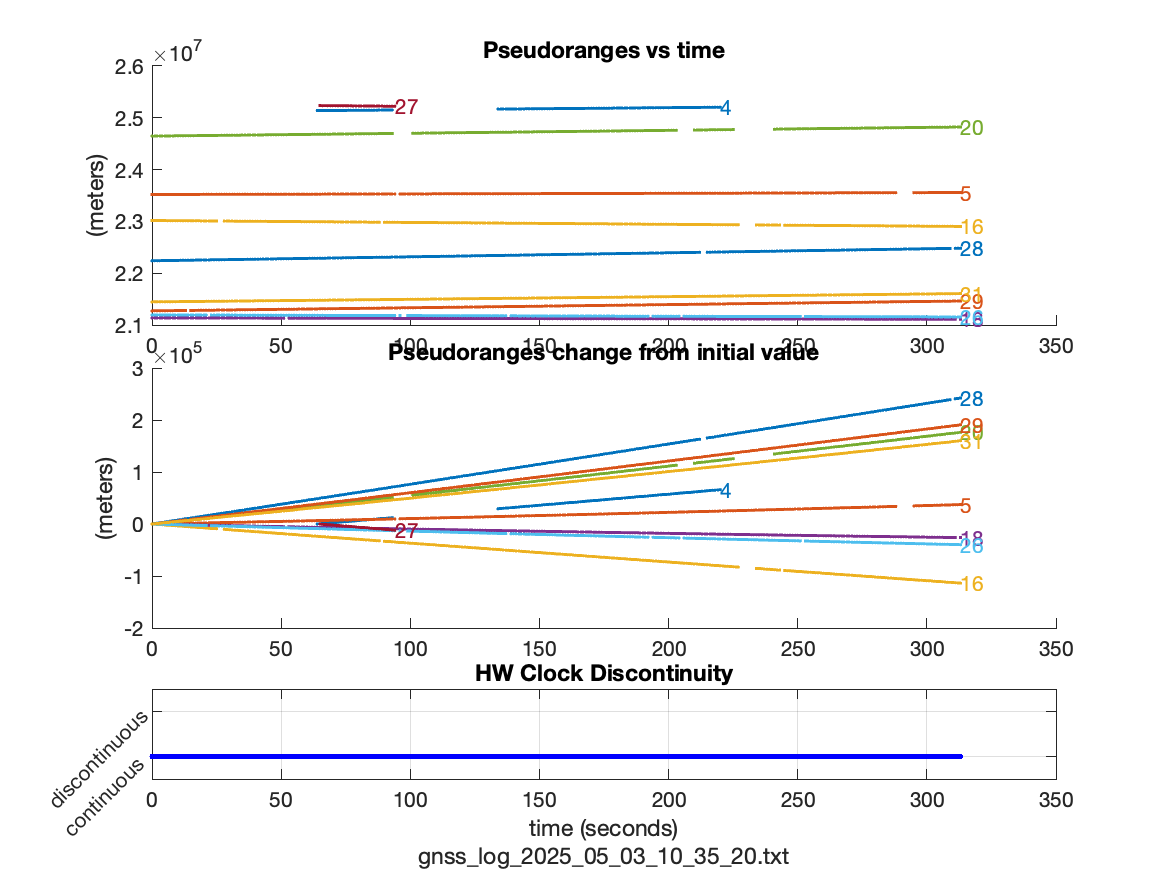
\includegraphics[width=\textwidth]{images/tests/Monte_Cappuccini/png/Samsung_A51_Monte_Cappuccini_fig1.png}
                \caption{Static: Pseudoranges vs time}
            \end{subfigure}
            \hfill
            \begin{subfigure}{0.23\textwidth}
                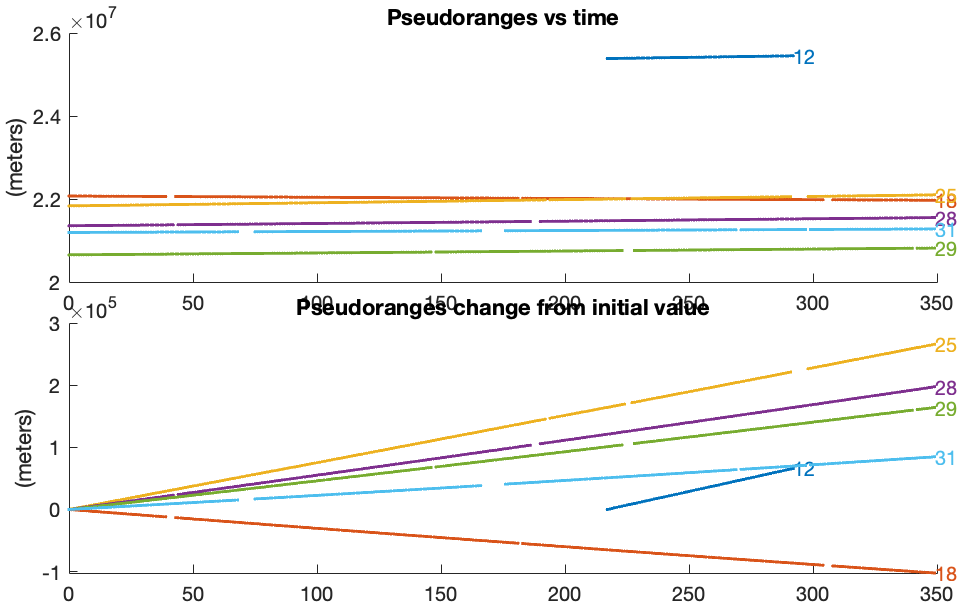
\includegraphics[width=\textwidth]{images/tests/Tram_15_trip_Castello_to_Pescatore/filtered/Samsung_A51_Tram_15_trip_Castello_to_Pescatore_fig1.png}
                \caption{Dynamic: Pseudoranges vs time}
            \end{subfigure}
        \end{figure}
    
        \vspace{0.5em}
        \textbf{Pseudorange Change from Initial Value.} 
        Expressing the measurements as a deviation from their epoch-0 value removes the common
        clock term and highlights the pure range-rate behaviour.  For the stationary receiver the
        change is almost perfectly linear; a best-fit slope gives range-rates of only a few
        \si{mm/s}, in line with the projection of the satellite’s
        ($\approx$\,\SI{3.9}{\kilo\metre\per\second}) velocity onto a fixed point on Earth.
        The difference between the derivative of the raw pseudorange and the reported
        pseudorange-rate (carrier Doppler observable) averages to
        $\lvert\bar{\Delta}\rvert<\SI{0.15}{\metre\per\second}$ for all tracked vehicles,
        confirming high internal consistency.\\[2pt]
        During the tram ride the same plot shows visibly larger, sometimes opposite-sign slopes
        that reach $\pm$\SI{3}{\metre\per\second}–\SI{4}{\metre\per\second}.
        These extra terms are simply the projection of the vehicle’s motion on the corresponding
        line-of-sight.  Because the receiver is accelerating, the straight-line assumption no
        longer holds perfectly and the residual between the differentiated pseudorange and the
        logged Doppler grows to $\approx$\SI{0.4}{\metre\per\second}–\SI{0.5}{\metre\per\second}
        for several satellites.  Short gaps in the traces translate into offsets in the cumulative
        curve, another indication of cycle slips or measurement drop-outs typical in a dynamic
        urban corridor.


        \begin{figure}[H]
            \centering
            \begin{subfigure}{0.23\textwidth}
                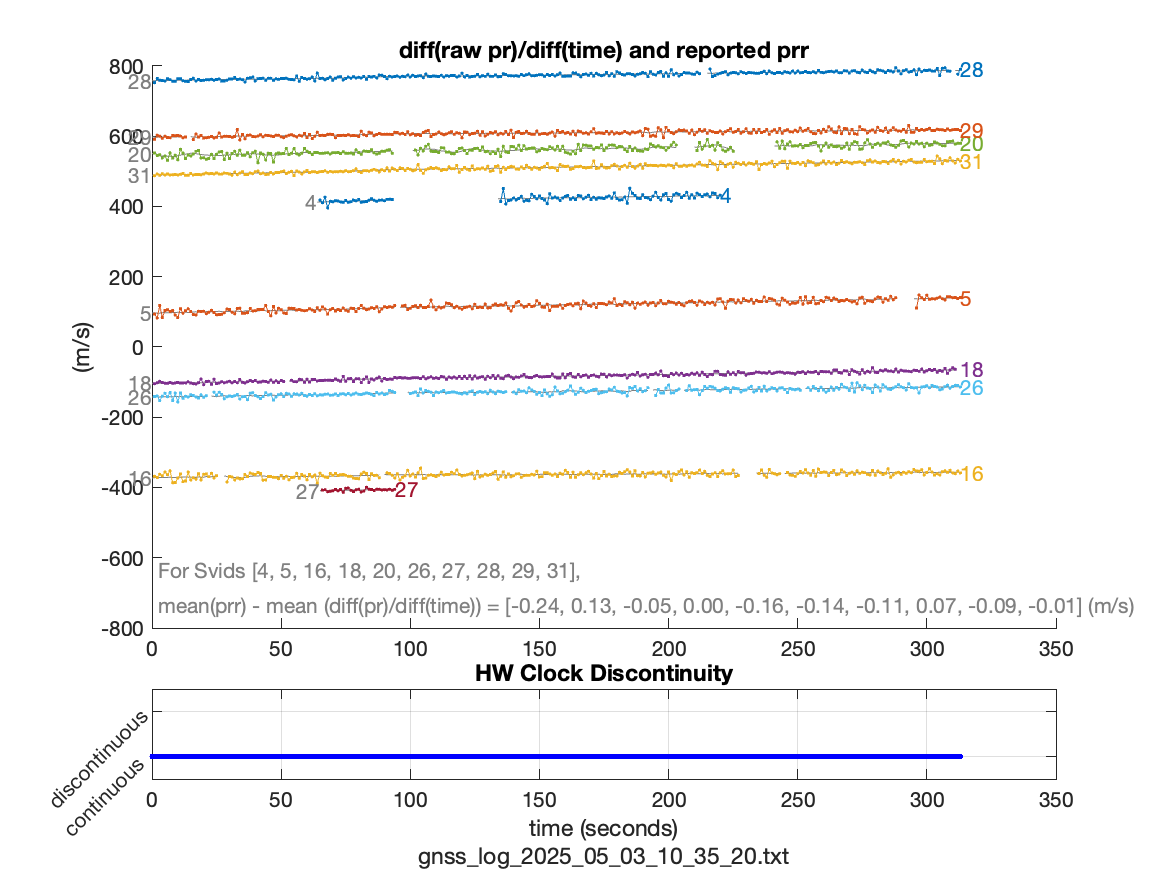
\includegraphics[width=\textwidth]{images/tests/Monte_Cappuccini/png/Samsung_A51_Monte_Cappuccini_fig2.png}
                \caption{Static: $\Delta$ Pseudorange}
            \end{subfigure}
            \hfill
            \begin{subfigure}{0.23\textwidth}
                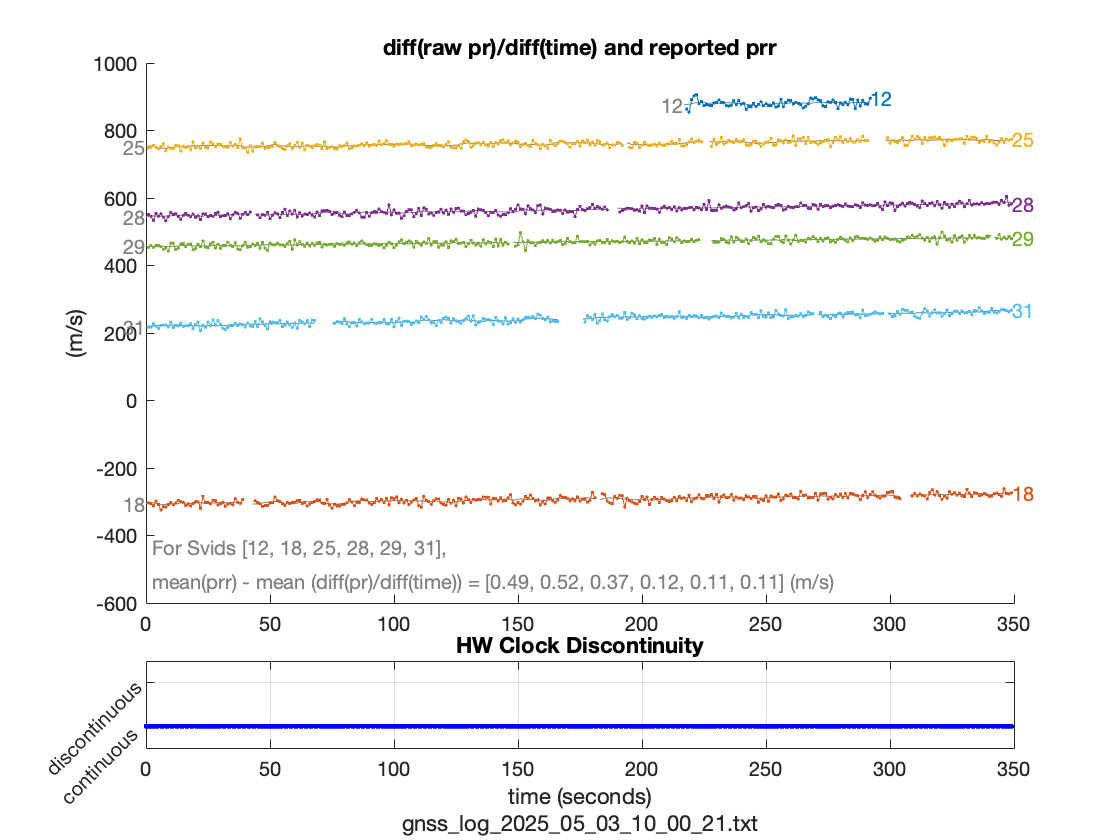
\includegraphics[width=\textwidth]{images/tests/Tram_15_trip_Castello_to_Pescatore/filtered/Samsung_A51_Tram_15_trip_Castello_to_Pescatore_fig2.png}
                \caption{Dynamic: $\Delta$ Pseudorange}
            \end{subfigure}
        \end{figure}
    
        \vspace{0.5em}
        \textbf{Positioning and Speed.} 
        The weighted-least-squares (WLS) solution for the static test forms a compact cloud
        centred only \SI{8}{\metre} (50 \% circle) around its median, a respectable accuracy for
        single-frequency raw-code positioning on a handset.  Horizontal speed never exceeds
        \SI{0.3}{\metre\per\second} and the HDOP stays below~1.2 while 7–9 GPS satellites are
        available, illustrating how good signal strength
        (C/No mostly 35–45 \si{dB\hertz}) and favourable geometry translate directly into a stable
        fix.\\[2pt]
        In the dynamic scenario the position scatter stretches along a NE--SW line that coincides
        with the real tram track.  Because the algorithm still assumes a static receiver, any
        un-modelled motion is interpreted as additional error: horizontal offsets reach several
        hundred metres and altitude shows a low-frequency bias.  The speed panel makes this
        clear—true tram velocities of 6–\SI{10}{\metre\per\second} are recovered, but frequent
        spikes up to \SI{20}{\metre\per\second} appear when the constellation drops to the legal
        minimum of four satellites or when strong multipath corrupts one of the ranges.
        HDOP occasionally climbs above~10 whenever a satellite is lost, amplifying the effect of
        the raw measurement noise.


        \begin{figure}[h!]
            \centering
            \begin{subfigure}{0.23\textwidth}
                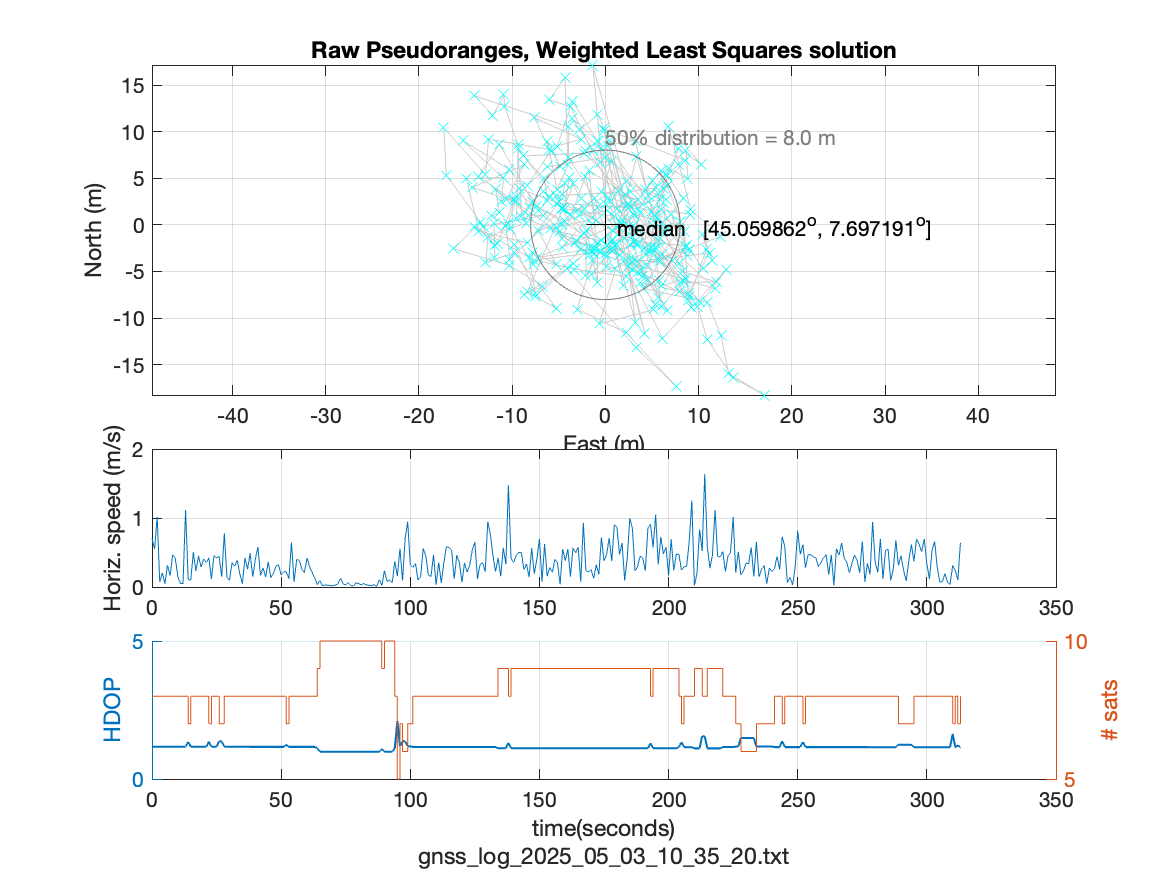
\includegraphics[width=\textwidth]{images/tests/Monte_Cappuccini/png/Samsung_A51_Monte_Cappuccini_fig4.png}
                \caption{Static: Position, Speed, HDOP}
            \end{subfigure}
            \hfill
            \begin{subfigure}{0.23\textwidth}
                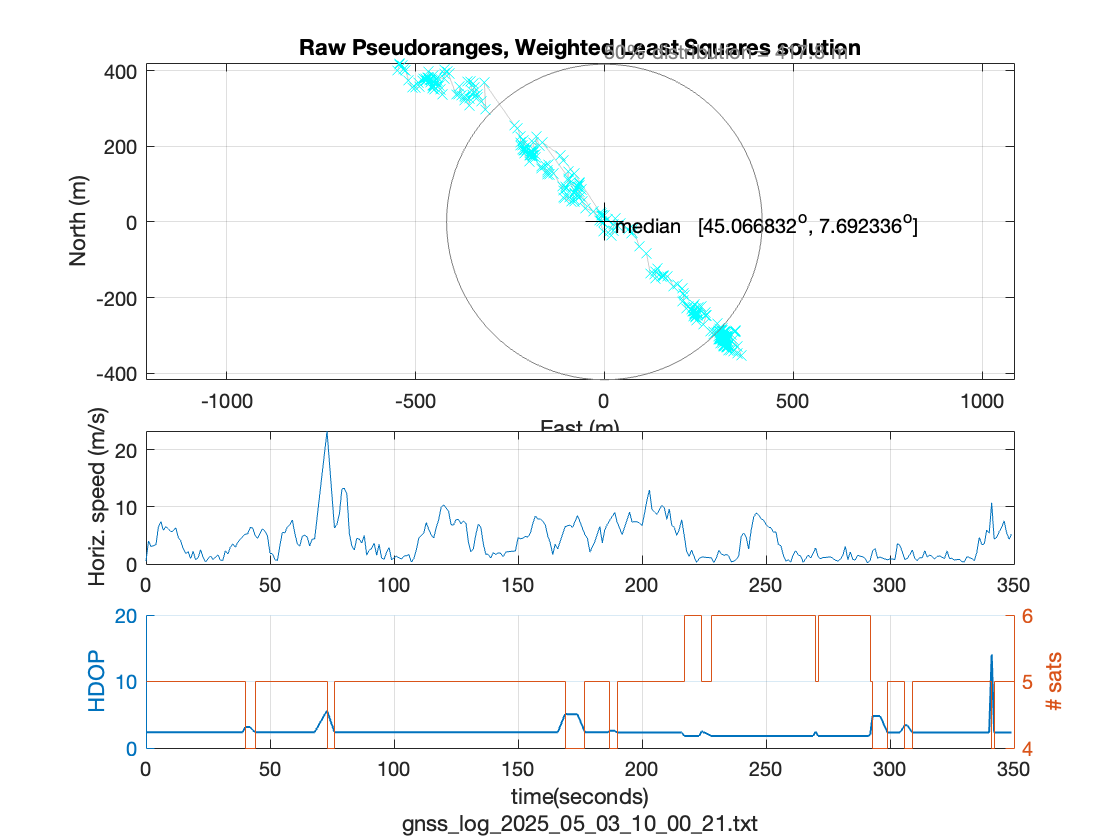
\includegraphics[width=\textwidth]{images/tests/Tram_15_trip_Castello_to_Pescatore/filtered/Samsung_A51_Tram_15_trip_Castello_to_Pescatore_fig4.png}
                \caption{Dynamic: Position, Speed, HDOP}
            \end{subfigure}
        \end{figure}
    
        \vspace{0.5em}
        \textbf{State Offsets and Timing Bias.} 
        For both logs the receiver clock bias grows almost linearly
        (about $2.4\times10^{4}$ \si{\metre}\,$\equiv$\,\SI{0.08}{\micro\second} over
        330 s), reflecting the free-running quartz error that is later absorbed by the WLS
        solution.  In static conditions the derived clock \emph{frequency} offset remains
        remarkably flat at $0.80\pm0.01$ \si{ppm}.  Once the phone is moving, self-heating,
        supply-voltage variation, and vibration induce a jitter five times larger; the
        instantaneous frequency estimate drifts between 0.70 and \SI{0.85}{ppm}.\\[2pt]
        Position-state residuals mirror the two use-cases: static latitude/longitude stay within
        $\pm$\SI{10}{\metre} and the vertical channel—traditionally the weakest—within
        $\pm$\SI{25}{\metre}.  When the tram starts, the solver sees continual geometry change;
        latitude and longitude offsets swing by $\pm$\SI{400}{\metre} while altitude error grows
        monotonically for several minutes before partially recovering.  Velocity states follow the
        true motion but also inherit short bursts produced by outlying pseudoranges.


        \begin{figure}[h!]
            \centering
            \begin{subfigure}{0.23\textwidth}
                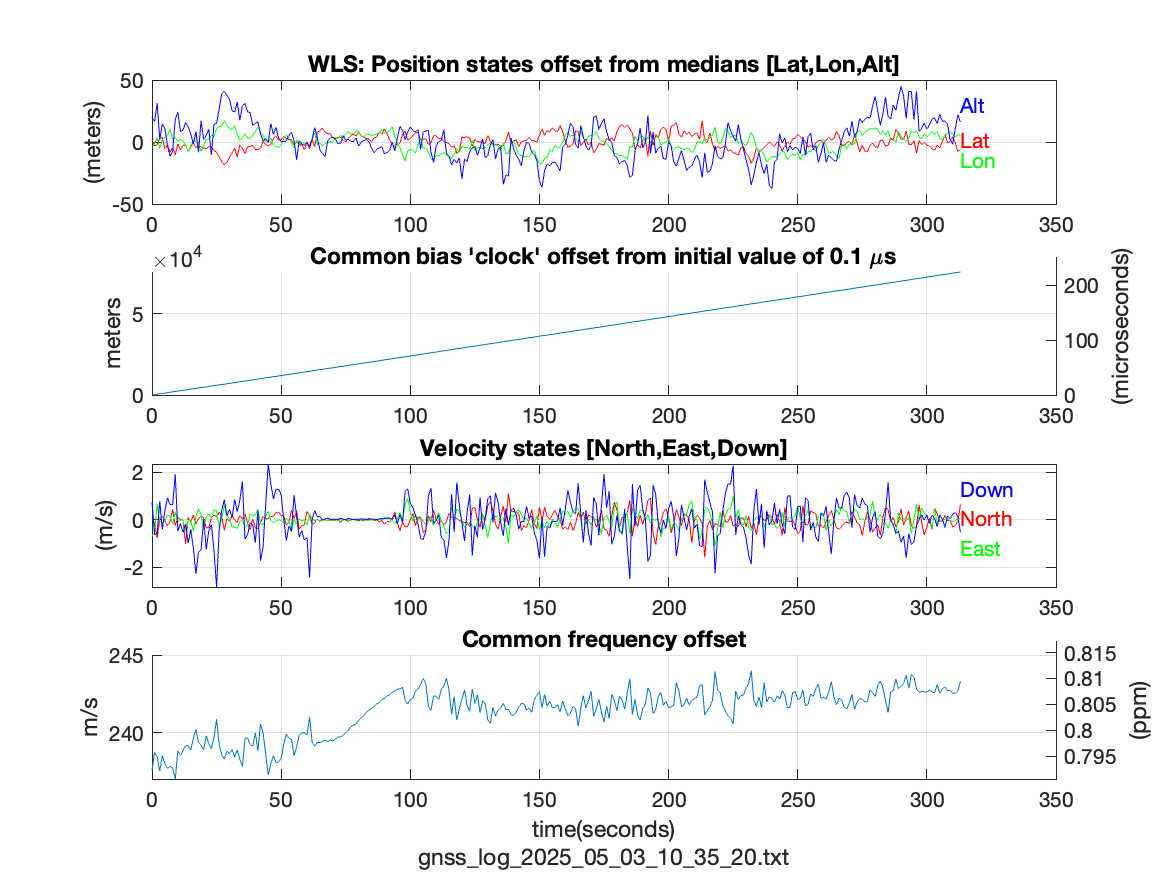
\includegraphics[width=\textwidth]{images/tests/Monte_Cappuccini/png/Samsung_A51_Monte_Cappuccini_fig5.png}
                \caption{Static: WLS states and bias}
            \end{subfigure}
            \hfill
            \begin{subfigure}{0.23\textwidth}
                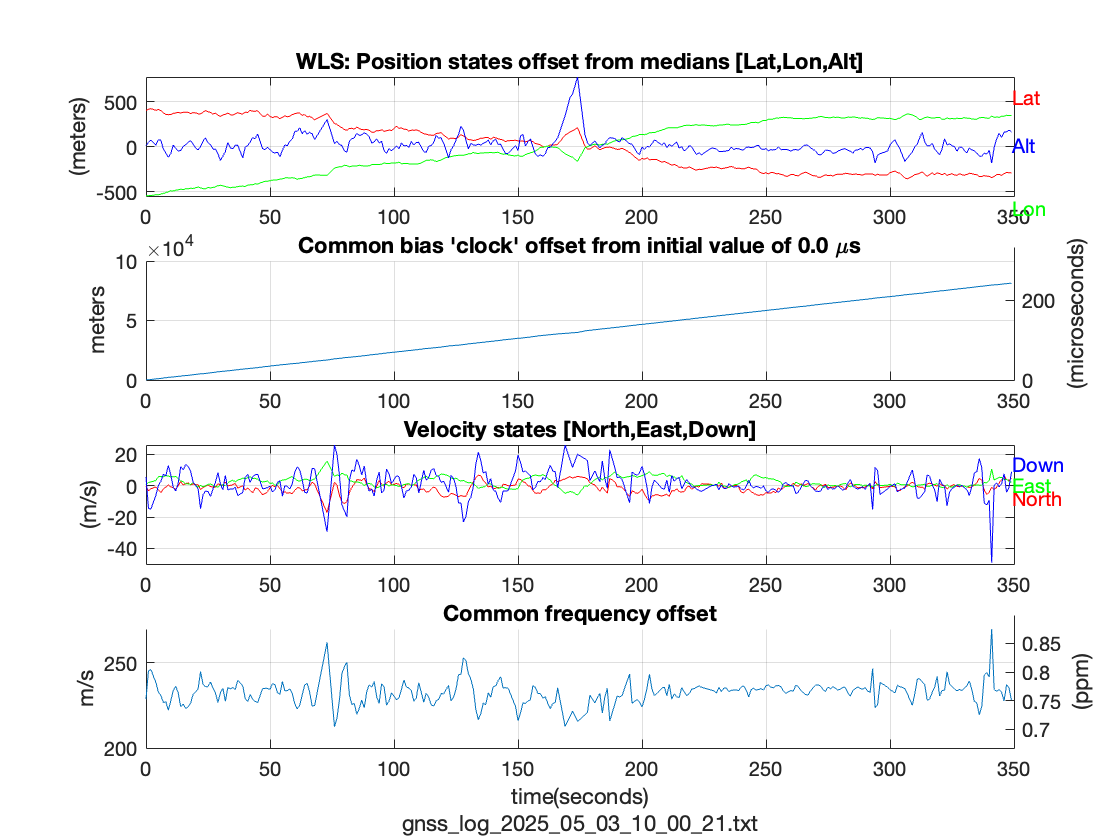
\includegraphics[width=\textwidth]{images/tests/Tram_15_trip_Castello_to_Pescatore/filtered/Samsung_A51_Tram_15_trip_Castello_to_Pescatore_fig5.png}
                \caption{Dynamic: WLS states and bias}
            \end{subfigure}
        \end{figure}
    
    \bigskip
    \noindent\textbf{Interpretation}\\
    The side-by-side analysis emphasises how a smartphone-grade GNSS front-end, although perfectly
    adequate for consumer navigation, is extremely sensitive to environment-induced dynamics when
    operated in raw-measurement mode:
    \begin{enumerate}
      \item \emph{Signal quality and tracking robustness} degrade once the antenna is surrounded by
            moving scatterers; this lowers C/No, increases the chance of cycle slips, and ultimately
            reduces the number of simultaneous measurements available to the PVT filter.
      \item \emph{Geometry} becomes a dominant error amplifier when only the minimum four satellites
            are left; every metre of code noise converts into several metres of position error as
            HDOP rises.
      \item \emph{Clock-oscillator behaviour} that looks perfectly linear at rest exhibits noticeable
            frequency wander when the handset experiences temperature cycling and mechanical stress.
      \item Finally, feeding a static-receiver WLS model with data collected in motion introduces a
            modelling mismatch that is clearly visible in the state-offset plots and should be
            corrected by switching to a dynamic filter (e.g.\ Kalman) or by incorporating external
            motion constraints.
    \end{enumerate}

    \medskip
    \noindent
    These findings highlight the importance of scenario-aware processing: identical hardware,
    firmware, and atmospheric conditions can yield centimetre-per-second stability on a quiet
    terrace, yet the very same setup will produce hundred-metre excursions once placed on a moving
    tram through an urban canyon.

    \subsection{Impact of Spoofed Position}

        In a spoofing attack, counterfeit signals are broadcast to mimic GNSS transmissions, often altering their timing, amplitude, or content. 
        Typically, these deceptive signals are sent at higher power than the originals to mislead navigation systems. 
        In our experiment, however, spoofing was implemented purely in software by adjusting the perceived reception time inside the professor’s script to simulate spoofing behavior.
            
        \noindent For the spoofed test we manually injected the coordinates of Piazza Vittorio Veneto (45.064749246294085, 7.6954660899754215) — a location adjacent to our true survey point — directly into the processing script. 
        As shown in the “Spoofed Case” plots (see attached PDF), this causes the solver to converge exactly at the Piazza Vittorio Veneto coordinates rather than the true measurement site, introducing a horizontal displacement of several hundred metres.
        
        \noindent Despite this spatial shift, all raw observables remain essentially unchanged relative to the normal run:
        
        \begin{itemize}
            \item \textbf{Carrier-to-noise density (C/N):} Histograms and time-series trace exactly overlap those of the baseline, confirming no change in received signal strength.
            \item \textbf{Dilution of precision (PDOP):} The satellite geometry quality curve is identical, indicating unchanged constellation geometry.
            \item \textbf{Pseudorange residuals:} The overall spread remains the same, but the entire residual distribution is offset by the constant delay corresponding to the spoofed displacement.
        \end{itemize}

        \begin{figure}[h!]
            \centering
            \begin{subfigure}{0.23\textwidth}
                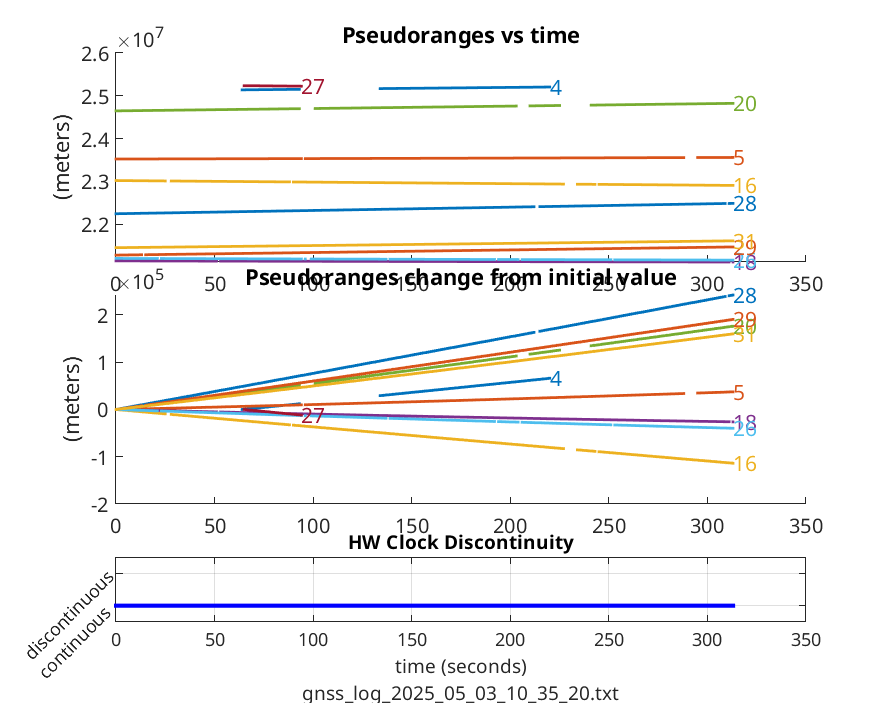
\includegraphics[width=\textwidth]{images/tests/Monte_Cappuccini/Spoofing/task5_figures/Samsung_A51_Monte_Cappuccini_fig1.png}
                \caption{Spoofed: Pseudoranges vs time}
            \end{subfigure}
            \hfill
            \begin{subfigure}{0.23\textwidth}
                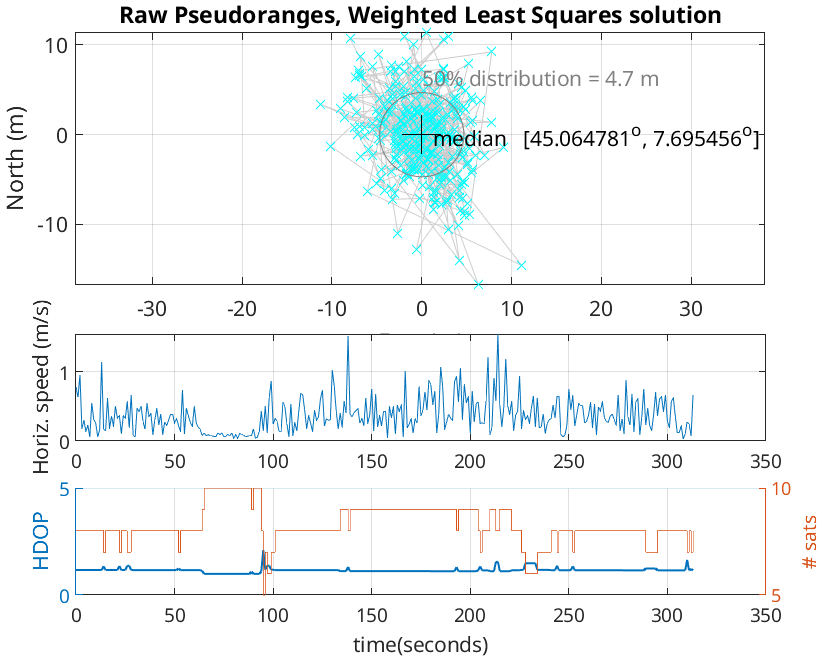
\includegraphics[width=\textwidth]{images/tests/Monte_Cappuccini/Spoofing/task5_figures/Samsung_A51_Monte_Cappuccini_fig4.png}
                \caption{Spoofed: Position, Speed, HDOP}
            \end{subfigure}
        \end{figure}


        \begin{figure}[h!]
            \centering
            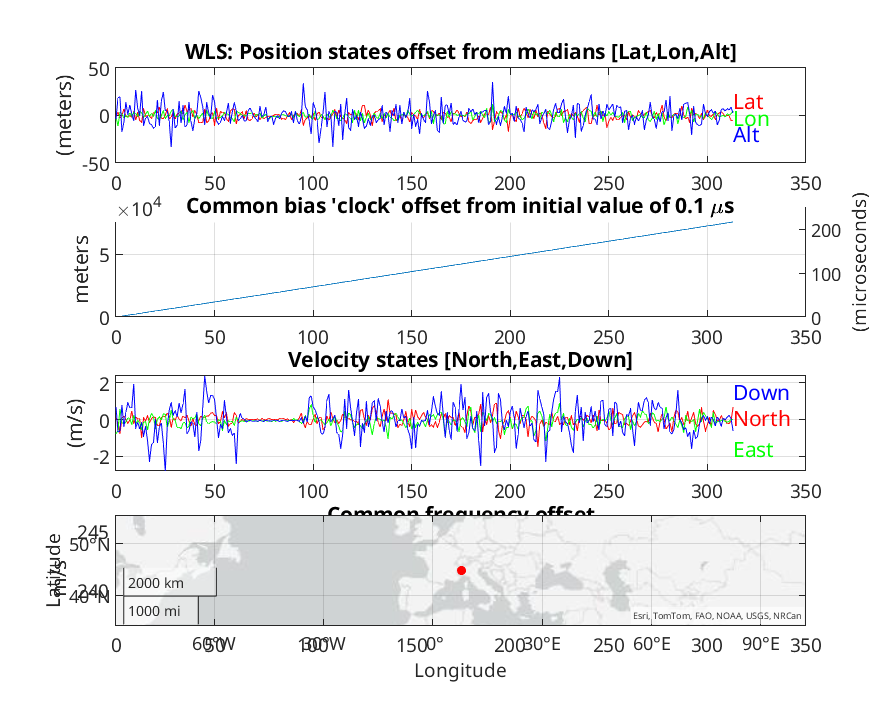
\includegraphics[width=0.9\columnwidth]{images/tests/Monte_Cappuccini/Spoofing/task5_figures/Samsung_A51_Monte_Cappuccini_fig5.png}
            \caption{Spoofed: WLS states and bias}
        \end{figure}

        
        \noindent Additionally, the 50\% (interquartile) range in the median-error distribution shrinks from approximately 8 m in the genuine case to about 4.7 m under spoofing. 
        This reduction occurs because the solver consistently “locks” onto the spoofed coordinate, decreasing variability around that false point.

    \subsection{Effects of Timing Delays}

        In this delayed-spoofing scenario we again target the same true survey point but now introduce a software-only replay delay: the spoofer “listens” to genuine signals, waits 1 ms, then injects the spoofed Piazza Vittorio Veneto coordinates starting at 50 s into the run. 
        The key parameters are set as:

        \begin{verbatim}
cfg.delay   = 1e-3;
cfg.t_start = 50;
        \end{verbatim}


        \begin{figure}[h!]
            \centering
            \begin{subfigure}{0.23\textwidth}
                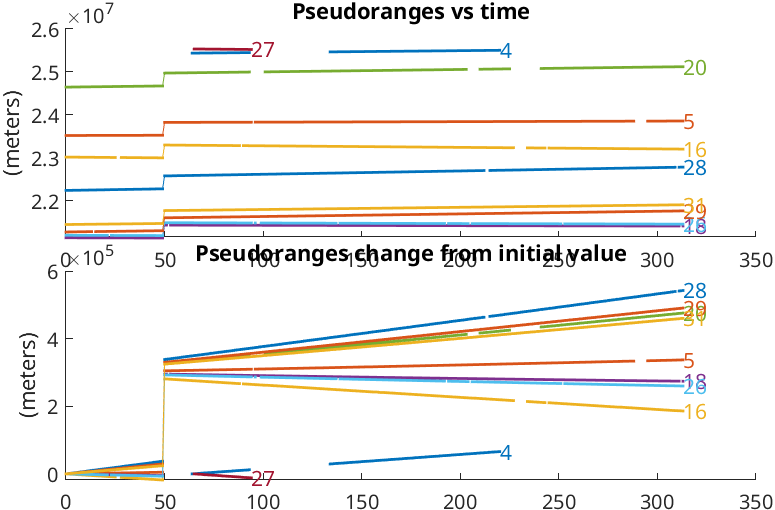
\includegraphics[width=\textwidth]{images/tests/Monte_Cappuccini/Spoofing/task6_figures/Samsung_A51_Monte_Cappuccini_fig1.png}
                \caption{Delay: Pseudoranges vs time}
            \end{subfigure}
            \hfill
            \begin{subfigure}{0.23\textwidth}
                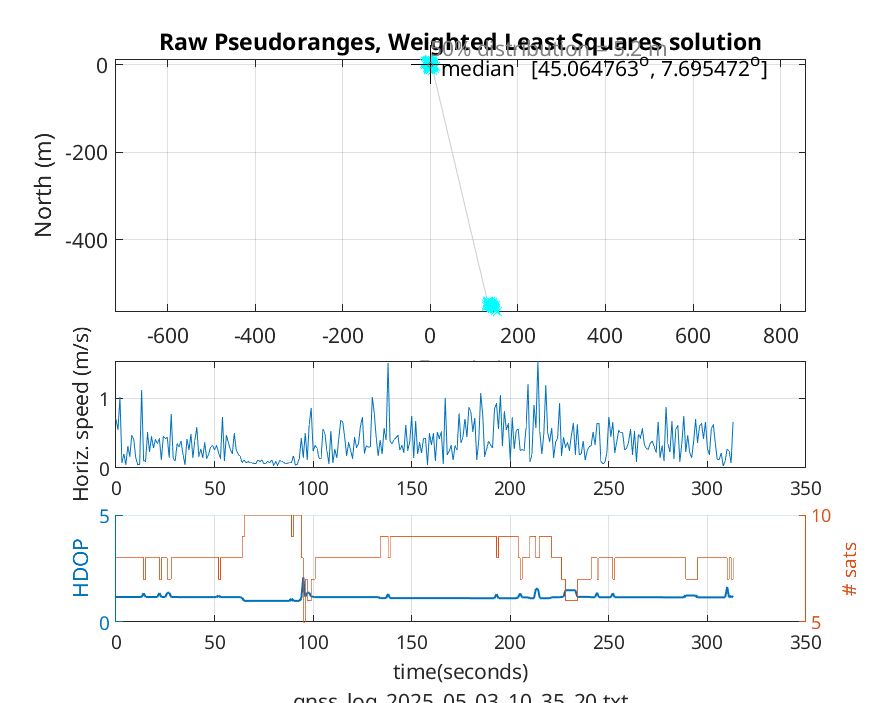
\includegraphics[width=\textwidth]{images/tests/Monte_Cappuccini/Spoofing/task6_figures/Samsung_A51_Monte_Cappuccini_fig4.png}
                \caption{Delay: Position, Speed, HDOP}
            \end{subfigure}
        \end{figure}

                \begin{figure}[h!]
            \centering
            \begin{subfigure}{0.23\textwidth}
                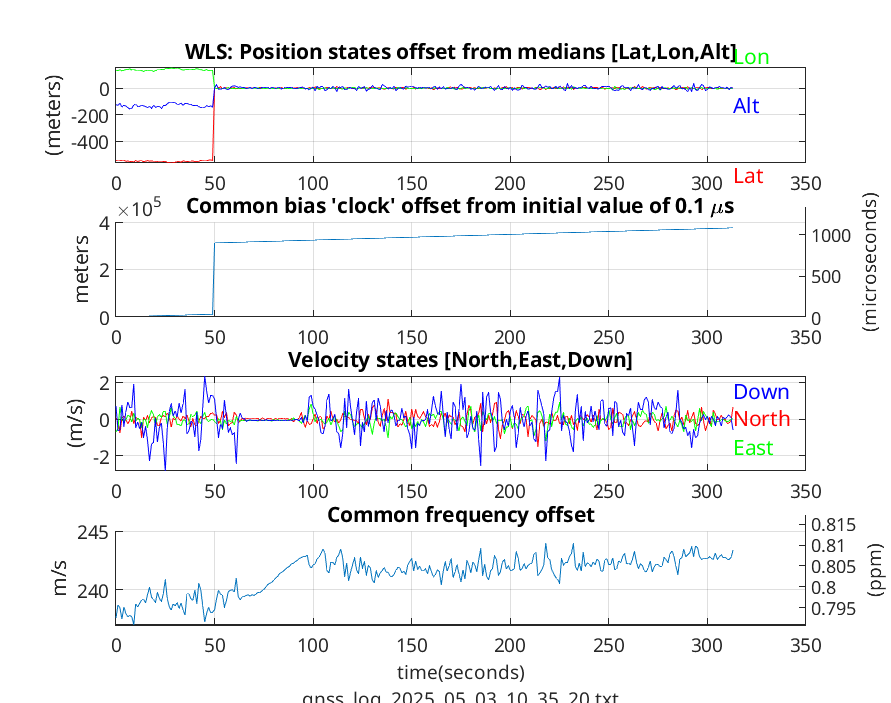
\includegraphics[width=\textwidth]{images/tests/Monte_Cappuccini/Spoofing/task6_figures/Samsung_A51_Monte_Cappuccini_fig5.png}
                \caption{Delay: WLS states and bias}
            \end{subfigure}
            \hfill
            \begin{subfigure}{0.23\textwidth}
                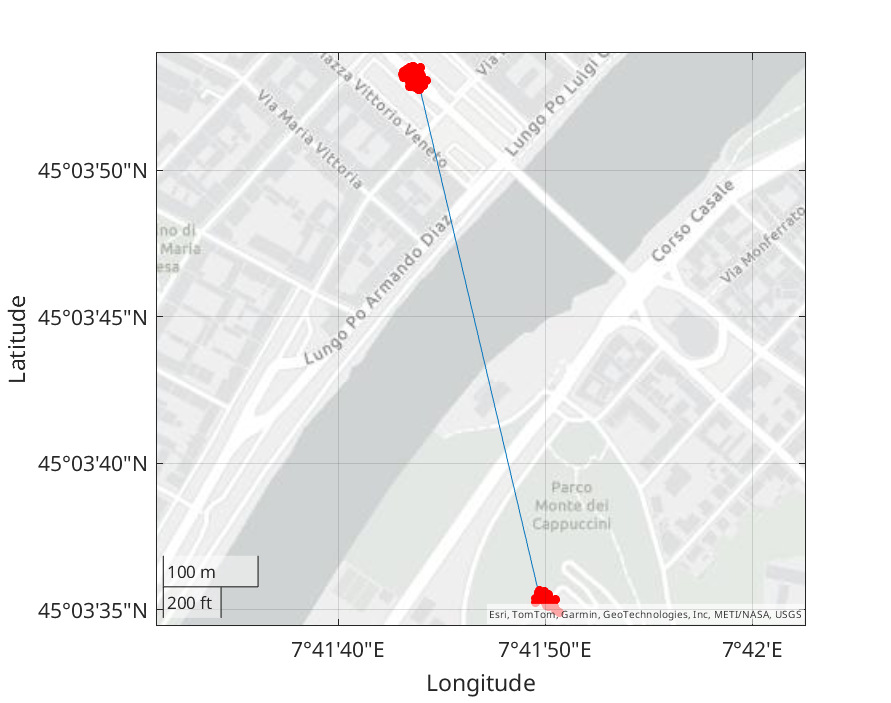
\includegraphics[width=\textwidth]{images/tests/Monte_Cappuccini/Spoofing/task6_figures/Samsung_A51_Monte_Cappuccini_fig6.png}
                \caption{Delay: Position}
            \end{subfigure}
        \end{figure}

        \noindent As visible in the plots, all observables remain nominal until t=50 s, at which point the solver's estimated position and receiver clock-bias exhibit a clear discontinuity as the spoof takes effect.

        \begin{itemize}
            \item \textbf{Position solution:} Prior to 50 s, the estimated coordinate coincides with the true static point. Immediately after 50 s, the solution jumps to the spoofed Piazza Vittorio Veneto location, replicating the static-spoof offset of several hundred metres.  
            \item \textbf{Receiver clock-bias:} A sudden step of appears in the estimated receiver clock-bias track, directly corresponding to the 1 ms replay delay needed to shift the range solution by the planar offset.  
            \item \textbf{Carrier-to-noise density (C/N):} The C/N time-series shows no amplitude change at t=50 s—signal strength is unaffected by delay.  
            \item \textbf{Dilution of precision (PDOP):} Satellite geometry quality remains continuous and invariant through the spoof onset.  
            \item \textbf{Pseudorange residuals:} Residuals maintain the same spread, but their mean shifts abruptly at 50 s by the additional delay delta t.  
        \end{itemize}
        
        \noindent From a solver-stability perspective, the sudden time bias causes an immediate step in both position and clock-bias, sometimes triggering a brief convergence glitch (extra iterations or loss of fix) as the estimator re-optimizes. 
        Even a 1 ms replay delay can therefore introduce a large positional error and matching clock-bias shift without altering any standard observables. Detecting such covert delay-based spoofing thus requires monitoring for timing discontinuities.

    \subsection{Interference Effects}
    
        % If performed, explain signal degradations, cycle slips, and accuracy loss

        % content
